\documentclass[a4paper,twoside]{article}

\usepackage{epsfig}
\usepackage{subfigure}
\usepackage{calc}
\usepackage{amssymb}
\usepackage{amstext}
\usepackage{amsmath}
\usepackage{amsthm}
\usepackage{multicol}
\usepackage{pslatex}
\usepackage{apalike}
\usepackage{SciTePress}

%\subfigtopskip=0pt
%\subfigcapskip=0pt
%\subfigbottomskip=0pt

\begin{document}
	
	\title{\uppercase{...}}
	
	\author{\authorname{Herval Bernice Nganya Nana\sup{1}}
		\affiliation{\sup{1}Fachbereich Informatik und Medien, Technische Hochschule Brandenburg, Deutschland}
		\email{nganyana@th-brandenburg.de}
	}
	
	\keywords{...}
	
	\abstract{...}{...}
	
	\onecolumn \maketitle \normalsize \vfill
	
	\section{\uppercase{Prototyp}}
	
	In diesem Kapitel geht es um die Beschreibung des Weges zur Erzeugung des ersten Produkts. Dieses wurde mittels der Werkzeuge Swagger \cite{swagger} (Swagger UI, Swagger Editor und Swagger Codegen), Amazon Web Services und Hibernate erarbeitet. F\"ur eine Modellgetriebene Entwicklung wurde w\"ahrend der Durchf\"uhrung dieses Projekts Bottom-Up entwickelt, sondern Top-Down. Also wurde direkt von angefertigten Modellen zum generierten Produkt enwickelt.
	
	\subsection{Funktionalit\"at}
	
	Da das Ziel des ganzen, urspr\"unglichen Projekts ein Anwendung zur Datenverwaltung ist. Das in dieser Dokumentation beschriebene Rest-Service, der daf\"ur verantwortlich ist Schnittstellen zu diesem Zweck bereitzustellen, erm\"oglicht:
	\begin{enumerate}
		\item einen Benutzer zu erstellen
		\item sich als Benutzer ein- und auszulogen
		\item Dateien hochzuladen, herunterzuladen, zu l\"oschen, umzubennenen und aufzulisten
		\item Ordner zu erstellen, zu l\"oschen, umzubennenen und zu visualisieren.
	\end{enumerate}
	
	Insgesamt sind von dem Rest-Service 11 Schnittstellen zur Verf\"ugung gestellt.
	
	\subsection{Schnittstellenerzeugung}
	
	Der Prozess zur Erzeugung der Schnittstellen ist in Folgende gelaufen:
	\begin{enumerate}
		\item zuerst wurden mittels des Werkzeugs Swagger Editor die Modelle, Schnittstellen sowie einpaar Meta-Daten des Projekts unter Anderen der Titel, die Beschreibung, die Version beschrieben. All das wird entweder unter einer JSON- oder YAML-Datei gespeichert. In diesem projekt wurde die JSON-Datei bevorzugt.
		
		\item Anschlie\ss{}end wurde aus dieser Beschreibung eine graphische Beschreibung der Schnittstellen als Webseite mittels Swagger UI erzeugt. Die enth\"alt einerseits die Schnittstellenbeschreibung andererseits die Modellbeschreibung.
		
		\item Dann wurde ebenfalls aus der JSON-Beschreibung der Quellcode anhand Swagger Codengen generiert. Swagger Codegen erm\"oglicht, den Quellcode in vielen Programmiersprachen (Backend sowie Frontend) zu erzeugen. F\"ur dieses Projekt wurde ein Spring-Projekt gew\"ahlt, da das angestrebte Produkt ein Rest-Service sein soll.
		
		\item Danach wurden in dem generierten Spring-Projekt Abh\"angigkeiten hinzugef\"ugt. Diese sind unter Anderen AWS S3, MySql und Spring-Data.
		
		\item Der n\"achste Schritt war dann die Verbindung zu der MySql-Datenbank und die Modelle gem\"a\ss{} der verschiedenen Attribute, die in der Datenbank zu speichern sind, zu annotieren. F\"ur dieses ist Hibernate zust\"andig.
		
		\item Abschlie\ss{}end wurde jede von Swagger automatisch generierte Funktion ausgef\"ullt. Bei der Generierung der Schnittstellen ist von Swagger eine leere Funktion pro Schnittstelle generiert. Es bleib nur noch diese Funktionen auszuf\"ullen.
	\end{enumerate}
	
	\subsection{Erweiterung der Schnittstellen (mit Datenbankerstellung)}
	
	Der Rest-Service k\"onnte noch Funktionalit\"aten bereitstellen, die in diesem Prototyp noch nicht entwickelt worden sind.
	
	\subsubsection{Encryption-M\"oglichkeit}
	In dem UserLogin-Modell ist ein Feld encryption so gedacht, dass die \"ubertragenen Daten vor der \"Ubertragung verschl\"usselt werden. Bei True sollen die Daten chiffriert werden und bei False nicht. \"Uber das Verschl\"usselungsverfahren soll sich der Entwickler entscheiden.
	
	\subsection{Rebuild des Projektes nach Schnittstellenbearbeitung}
	
	Das Projekt wird basiert auf einer Menge von Schritten nach und nach durchgeführt. Gleich nach der Beschreibung der Modelle und der Schnittstellen bis zum generierten Projekt wird jede Code-Zeile automatisch generiert. Was ist denn, zu tun, falls Änderungen in der Beschreibung vorkommen? Der neu generierte Code soll integriert werden, ohne den bereit Selbstgeschriebene Code zu überschreiben. Zu diesem Zweck werden in dem Paper \cite{timo2015} ein paar Methoden vorgestellt, die in solchen Fällen nützlich sind. Im Rahmen dieser Arbeit wurde aus Zeitgründen keine dieser Methoden implementiert, aber eine davon hat sich trotzdem durch die fünf von diesem Paper vorgestellten Kriterien zu diesem Projekt passend gezeigt. Die heißt Generation Gap \cite{timo2015_3_1}.
	Bei diesem Verfahren werden beispielsweise für eine Klasse NotePad ein Interface NotePad und eine Standard-Implementierung NotePadBaseImpl generiert. Diese Klasse zur Implementierung unterscheidet sich von der eigenen Implementierung, die zum Beispiel in der Klasse NotePadImpl geschrieben ist, in sofern als die dazu gehörigen Codes unterschiedlich sind und die Klasse NotePadImpl wird zusätzlich bei einer neuen Erzeugung des Codes nicht überschrieben (Abbildung \ref{fig:generation-gap-muster-für-das-notepad-beispiel}). NotePadImpl ist die Implementierung, die von beiden Codes (der generierte und der Selbstgeschriebene) verwendet werden soll.
	
	Gründe für die Wahl dieser Methode ist:
	\begin{enumerate}
		\item Die Struktur des endgültigen Quellcodes in diesem Projekt weicht nur von dem ursprünglichen Code um die Pakete io.swagger.service, io.swagger.repository, io.swagger.configuration. Ähnlich NotePadImpl in \cite{timo2015_3_1} sind die Klassen wie FileService, FolderService und UserService die Selbstgeschriebenen Klassen, die nicht überschrieben werden sollten. Dies erfüllt das Kriterium C1.
		
		\item Die anderen Klassen in io.swagger.api, io.swagger.api, io.swagger.model und io.swagger sind hier generierte pakete. Ihre Inhalte können beliebig überschrieben werden. Das Kriterium C2 ist erfüllt.
		
		\item Die generierten Schnittstellen können im Laufe des Projekt erweitert werden, ohnen den Selbstgeschriebenen Code zu beeinflüssen.  Das Kriterium C3 ist erfüllt.
		
		\item Das Kriterium C4 ist ebenfalls erfüllt, da der Selbstgeschriebene Code unabhängig von dem generierten Code ist. Dies ist auf die Tatsache, dass der generierte Code keinen Einfluss auf den Selbstgeschriebenen hat.
		
		\item In diesem Projekt wurde der Code in Spring (Java) generiert. Nach einer neuen Erzeugung ist der generierte Code immernoch auf die gleiche Programmiersprache. Dies fordert deshalb keine zusätzliche Programmiersprache. So ist das Kriterium C5 erfüllt.
	\end{enumerate}
	
	\begin{figure}[ht]
		\centering
		{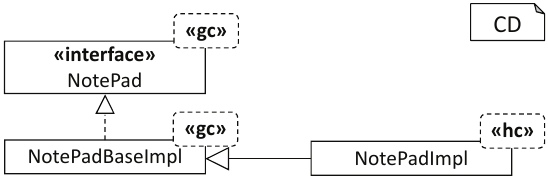
\epsfig{file = generation_gap.png, width = 7.5cm}}
		\caption{Generation Gap Muster für das NotePad-Beispiel\\ gc: generated code, hc: hand code}
		\label{fig:generation-gap-muster-für-das-notepad-beispiel}
	\end{figure}
	
	\section{Ergebnisse und Probleme}
	
	\subsection{Ergebnisse}
	
	Schlie\ss{}lich liegt nach einer Schritt f\"ur Schritt Arbeitsweise der gezielte Rest-Service vor. Der ist in der Lage die 11 Funktionalit\"aten anzubieten, die vorher angek\"undigt waren. Die Daten sind dank einer Datenbank und einer Speicherung der auf AWS S3 tats\"achlich persistent. Der Rest-Service kann ebenfalls entsprechende Antworten zur\"uckgeben:
	\begin{enumerate}
		\item 400 Bad Request
		\item 403 Forbidden
		\item 404 Not Found
	\end{enumerate}
	
	\subsection{Probleme}
	
	W\"ahrend der Entwicklung ist das Team auf Schwierigkeiten gesto\ss{}en. Diese waren einerseits aufgrund der Verwendung eines Modellgetriebene-Software-Entwicklungswerkzeugs ausgel\"ost andererseits aufgrund der Datensicherheit bei der Nutzung vom AWS S3.
	
	\subsubsection{Un\"ubersichtlicher, generierter Code}
	
	Der von Swagger generierte Code l\"asst ist an vielen Stellen kaum \"ubersichtlich. Der Code in den Kontrollern und Interfaces ist schwer zu verstehen  (Abbildung \ref{fig:quellcode-der-schnittstellen-getFile-und-editFile}). 
	
	\begin{figure}[ht]
		\centering
		{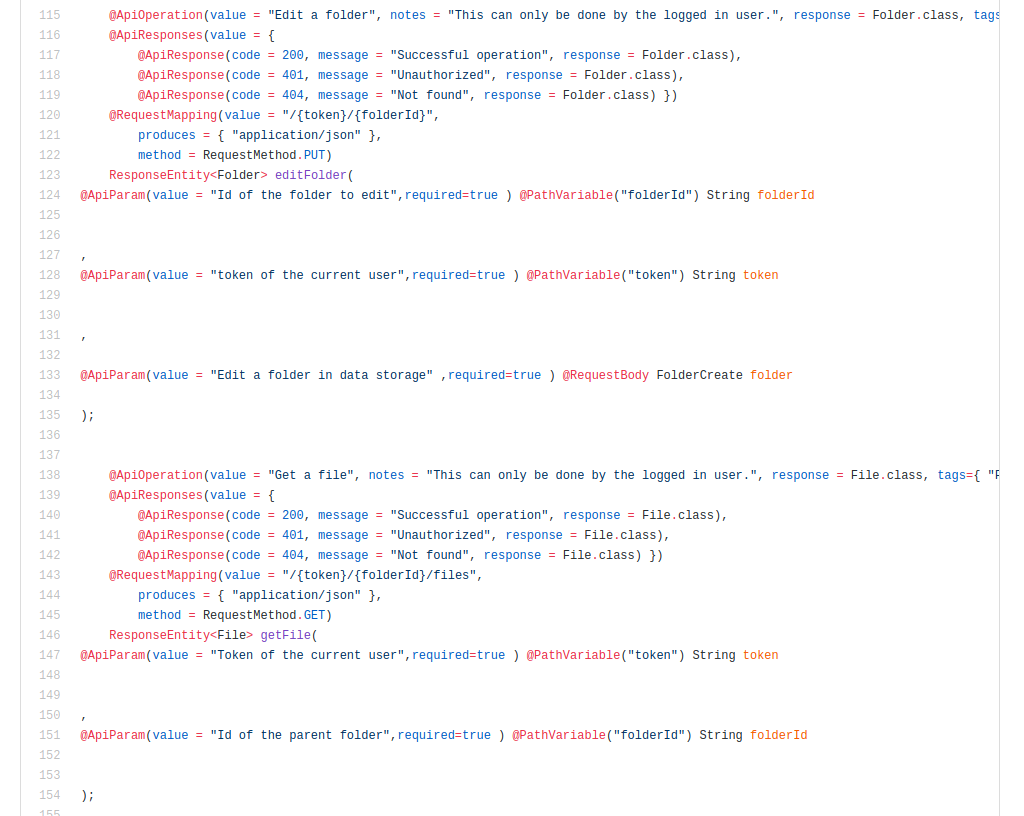
\epsfig{file = interfaces.png, width = 8cm}}
		\caption{Quellcode der Schnittstellen getFile und editFile}
		\label{fig:quellcode-der-schnittstellen-getFile-und-editFile}
	\end{figure}
	
	\subsubsection{Projektstruktur}
	
	Nach Entwicklern oder Organisationen kann die Paketestruktur variieren. Daher ist die von Swagger angebotene Paket Struktur  immer auf dem ersten Blick ungew\"ohnt (Abbildung \ref{fig:von-swagger-generierte-paketstruktur}). In dieser Abbildung ist das Paket io.swagger.service nicht von Swagger sondern von dem Entwicklungsteam generiert.
	
	\begin{figure}[ht]
		\centering
		{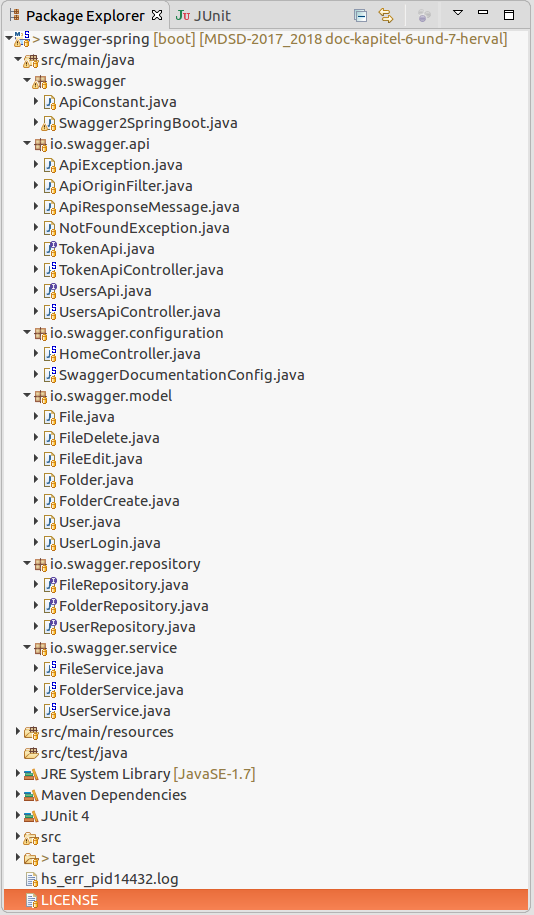
\epsfig{file = paketstruktur.png, width = 8cm}}
		\caption{Von Swagger generierte Paketstruktur}
		\label{fig:von-swagger-generierte-paketstruktur}
	\end{figure}
	
	\subsubsection{Sicherheit}
	
	AWS bietet den S3-Dient an, der erm\"oglicht Dateien auf dem Cloud zu speichern. Dies erfolgt per Quellcode mittels Access- und Secret-Keys. Damit das Team Trasaktionen mit S3 w\"ahrend der Entwicklung durchf\"uren kann, soll es diese Schl\"ussel besitzen. Das Problem ist an der Stelle die Verteilung dieser Schl\"ussel. Diese kann zu bosen Zwecken verwendet werden und schlie\ss{}lich hohe Kosten f\"ur den offiziellen Besitzer verursachen. Au\ss{}erdem w\"aren sie \"offentlich f\"ur Hackers durch GitHub gewesen, da GitHub zur Versionsverwaltung verwendet wurde.
	Aus diesen Gr\"unden wurde ein Nexus-Repository entwickelt und geheim gehalten, damit diese Access- und Secret-Keys nicht \"uberall stehen. Dieses Repository stellt ein Object S3Transaction zur Verf\"ugung, das seinerseits Funktionen wie upload, rename und delete zur Verf\"ugung stellt. Die S3Transaction-Abh\"angigkeit ist anhand des Folgenden aufzurufen:
	
	\begin{small}
		\begin{verbatim}
		<dependency>
		<groupId>
		com.mdsd-2017-2018.s3-transactions
		</groupId>
		<artifactId>
		s3-transactions
		</artifactId>
		<version>1.2.2</version>
		</dependency>
		\end{verbatim}
	\end{small}
	
	\vfill
	\bibliographystyle{apalike}
	{\small
		\bibliography{quellen}}
	
	\listoftables
	
	\listoffigures
\end{document}

